\chapter{\ac{UI} Design}\label{ch:ui-design}
Das \ac{UI} Design wird in mehreren Schritten erstellt und im Laufe des Projekts immer weiter
verfeinert. Am Anfang dieses Prozesses steht ein Low Fidelity Prototyp der Applikation.
Dieser dient dazu, das ungefähre Layout zu visualisieren und ein Gefühl für den Aufbau
des Frontends zu vermitteln. %eventuell etwas umgansprachlich schaffen -> vermitteln?%
Für die Erstellung dieser Prototypen wird die Prototyping- und
Designsoftware Figma \footnote{Software zum Erstellen von Softwareprototypen https://www.figma.com} verwendet.
%Figma mit fußnote oder Tool Liste?%

\section{Low Fidelity}\label{Low Fidelity}
\begin{figure}[h]
  \centering
    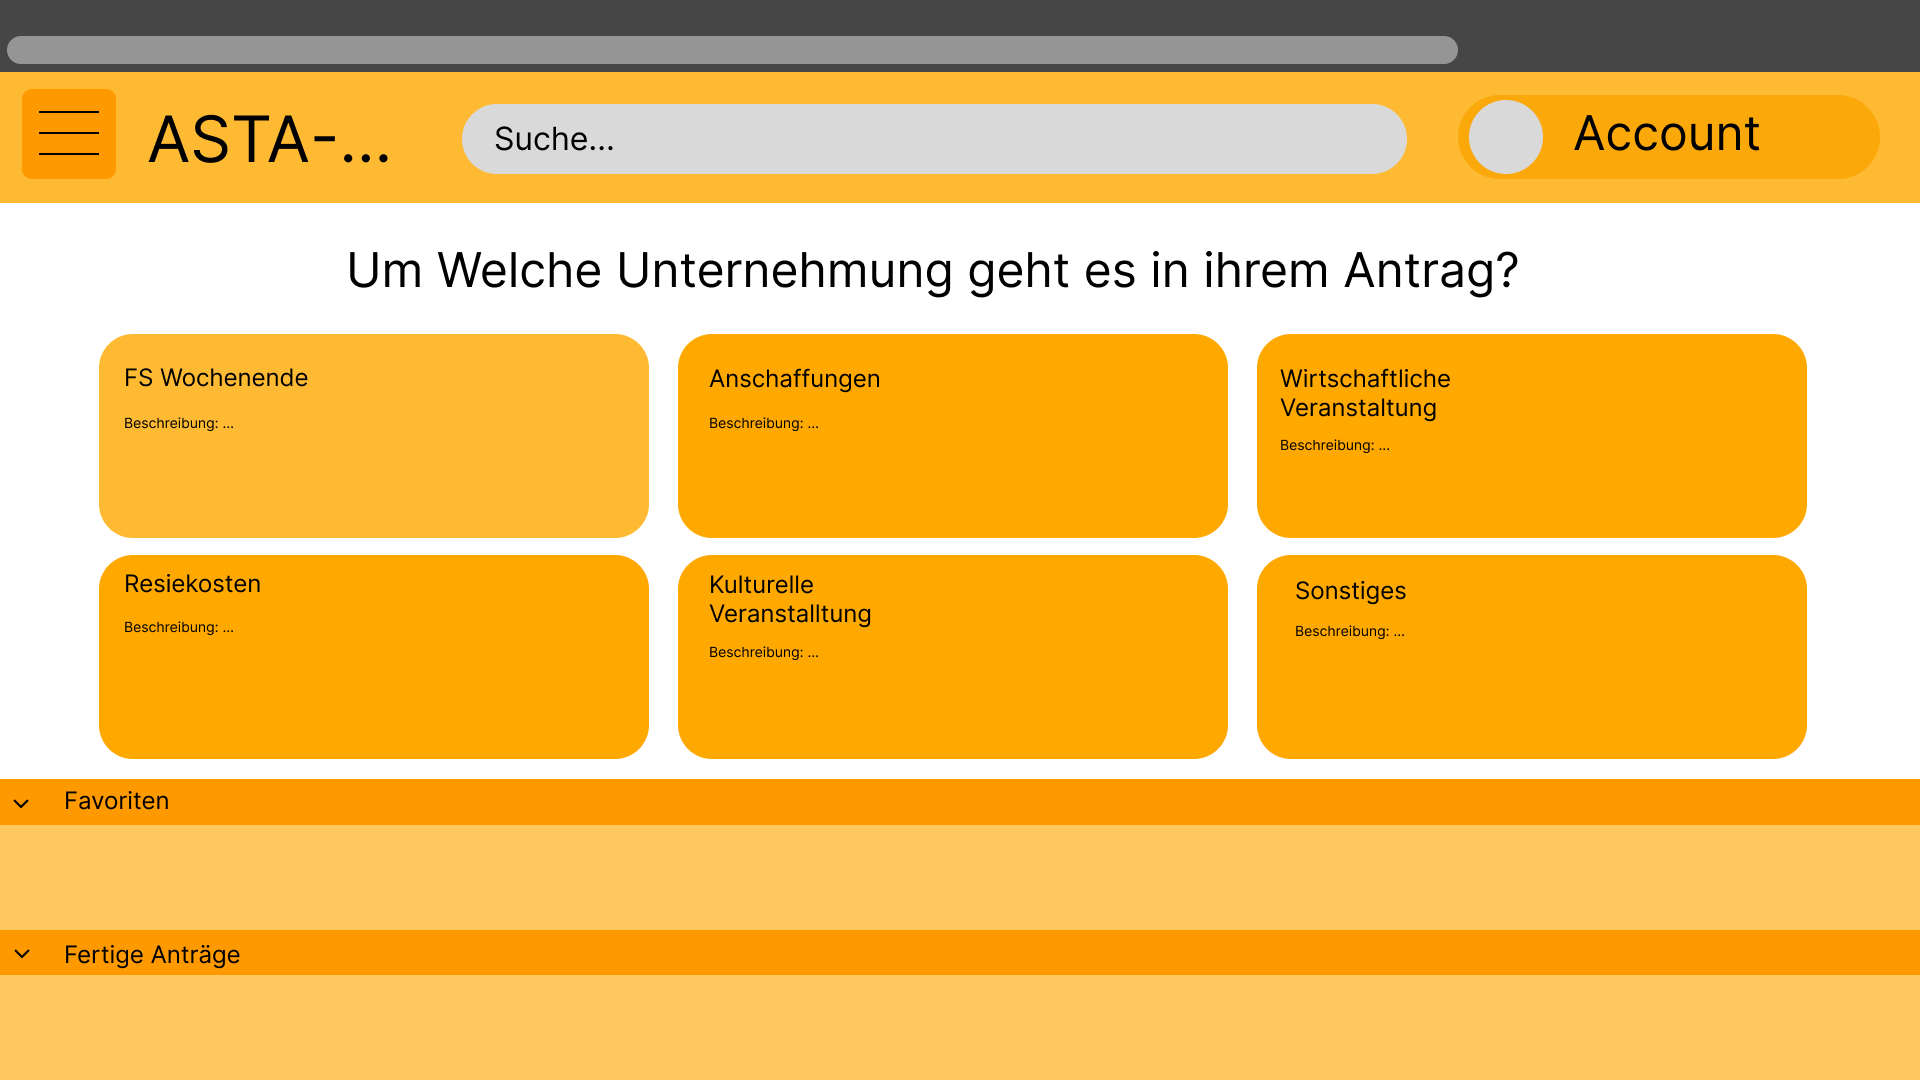
\includegraphics[width=1.0\textwidth]{Antragshelfer}
    \caption{Antragshelfer}\label{Antragshelfer}
\end{figure}
Das Layout des Prototyps lässt sich in drei Bereiche einteilen:
die Kopfzeile, den Hauptinhalt der Seite und die Fußzeile.

In der Kopfzeile befindet sich das \ac{AStA}-Logo, sowie eine Suchleiste um manuell nach
Anträgen zu suchen.
Auch der jeweiligen Nutzeraccount lässt sich über die Schaltfläche
am rechten Rand erreichen.
Außerdem befindet sich am linken Rand ein Burger-Menü,
welches das Hinzufügen von Funktionalitäten in zukünftigen Projekten erleichtern soll.

Der Hauptinhalt der Seite zeigt die Hauptfunktionalitäten unserer Anwendung und wird 
dynamisch generiert. Bei den Prototypen wird dies
durch ein statisches Layout simuliert.

Durch die Fußzeile soll der Nutzer die Möglichkeit erhalten, schnell und einfach auf
seine zuvor festgelegten Favoriten zugreifen zu können.
Was zu einer besseren User Experience führen soll.
Die Kopf- und Fußzeile der Applikation ist auf jeder Seite identisch.

Der Antragshelfer ist eine Hauptfunktionalität unserer Applikation deshalb fungiert
dieser als Landing-Page, wie in \refa{Antragshelfer} dargestellt.

Hier soll der Nutzer die ihm, von der Applikation gestellten, Fragen beantworten,
um so zum richtigen Antrag zu gelangen. %TODO Satz umvormoliren%
Die Beantwortung der Fragen erfolgt durch Klicken auf die verschiedenen Buttons. %Passt das so?%
Zur Übersicht, ist jeder Button mit einer Beschreibung versehen, welche genauere Informationen über die Auswahloption liefert.

\begin{figure}[h]
  \centering
    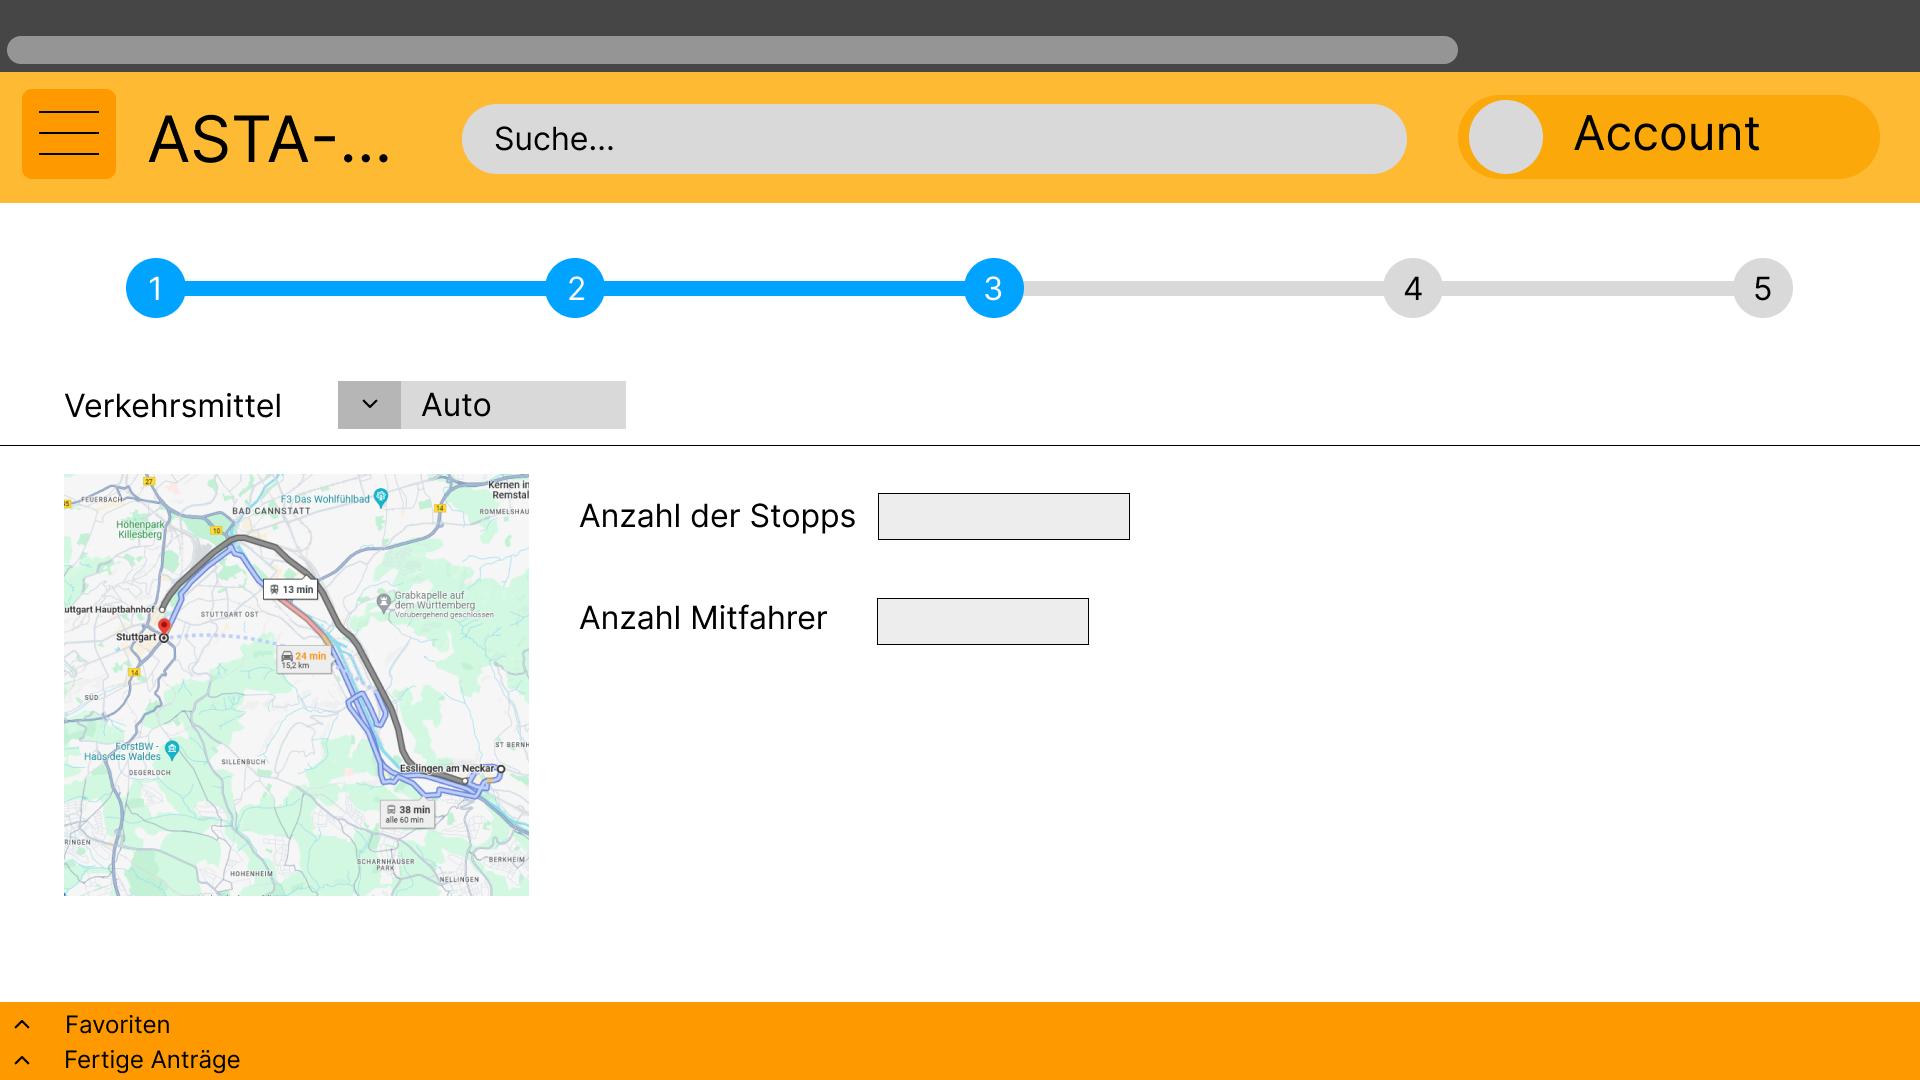
\includegraphics[width=1.0\textwidth]{Reisekostenhelper}
    \caption{Reisekostenhelfer}\label{Reisekostenhelfer}
\end{figure}


Beim Ausfüllen des Antrags hat der Nutzer die Möglichkeit über unterschiedliche Eingabemöglichkeiten,
wie Textfelder, Dropdown Menüs oder Checkboxen die benötigten Informationen einzugeben. Auch die Eingabe
über die integrierten \ac{API}s ist möglich, wie in \refa{Reisekostenhelfer} am Beispiel eines Reisekosten Antrags zu sehen.
Um dem Nutzer einen Überblick über den Fortschritt beim Ausfüllen des Antrags zu ermöglichen, befindet sich am oberen 
Rand eine Fortschrittsanzeige.
So soll der Nutzer darüber informiert werden, wie viele Schritte noch
nötig sind, bis der Antrag fertig bearbeitet ist. 







